% Template for Cogsci submission with R Markdown

% Stuff changed from original Markdown PLOS Template
\documentclass[10pt, letterpaper]{article}

\usepackage{cogsci}
\usepackage{pslatex}
\usepackage{float}
\usepackage{caption}

% amsmath package, useful for mathematical formulas
\usepackage{amsmath}

% amssymb package, useful for mathematical symbols
\usepackage{amssymb}

% hyperref package, useful for hyperlinks
\usepackage{hyperref}

% graphicx package, useful for including eps and pdf graphics
% include graphics with the command \includegraphics
\usepackage{graphicx}

% Sweave(-like)
\usepackage{fancyvrb}
\DefineVerbatimEnvironment{Sinput}{Verbatim}{fontshape=sl}
\DefineVerbatimEnvironment{Soutput}{Verbatim}{}
\DefineVerbatimEnvironment{Scode}{Verbatim}{fontshape=sl}
\newenvironment{Schunk}{}{}
\DefineVerbatimEnvironment{Code}{Verbatim}{}
\DefineVerbatimEnvironment{CodeInput}{Verbatim}{fontshape=sl}
\DefineVerbatimEnvironment{CodeOutput}{Verbatim}{}
\newenvironment{CodeChunk}{}{}

% cite package, to clean up citations in the main text. Do not remove.
\usepackage{apacite}

% KM added 1/4/18 to allow control of blind submission
\cogscifinalcopy

\usepackage{color}

% Use doublespacing - comment out for single spacing
%\usepackage{setspace}
%\doublespacing


% % Text layout
% \topmargin 0.0cm
% \oddsidemargin 0.5cm
% \evensidemargin 0.5cm
% \textwidth 16cm
% \textheight 21cm

\title{A large-scale comparison of cross-situational word learning
models}

\usepackage{booktabs}
\usepackage{longtable}
\usepackage{array}
\usepackage{multirow}
\usepackage{wrapfig}
\usepackage{float}
\usepackage{colortbl}
\usepackage{pdflscape}
\usepackage{tabu}
\usepackage{threeparttable}
\usepackage{threeparttablex}
\usepackage[normalem]{ulem}
\usepackage{makecell}
\usepackage{xcolor}

\author{{\large \bf George Kachergis (kachergis@stanford.edu)} \and {\large \bf Michael C.~Frank (mcfrank@stanford.edu)} \\ Department of Psychology, 450 Jane Stanford Way \\ Stanford, CA 94305 USA}

\newlength{\cslhangindent}
\setlength{\cslhangindent}{1.5em}
\newenvironment{CSLReferences}%
  {}%
  {\par}

\begin{document}

\maketitle

\begin{abstract}
One problem language learners face is extracting word meanings from
scenes with many possible referents. Despite the ambiguity of individual
situations, a large body of empirical work shows that people are able to
learn cross-situationally when a word occurs in different situations.
Many computational models of cross-situational word learning have been
proposed, yet there is little consensus on the main mechanisms
supporting learning, in part due to the profusion of disparate studies
and models, and lack of systematic model comparisons across a wide range
of studies. This study compares the performance of several extant models
on a dataset of 44 experimental conditions and a total of 1,696
participants. Using cross-validation, we fit multiple models
representing theories of both associative learning and
hypothesis-testing theories of word learning, find two best-fitting
models, and discuss issues of model and mechanism identifiability.
Finally, we test the models' ability to generalize to additional
experiments, including developmental data.

\textbf{Keywords:}
cross-situational word learning; model comparison; language learning
\end{abstract}

\hypertarget{introduction}{%
\section{Introduction}\label{introduction}}

Learning word meanings is a crucial aspect of the process of language
acquisition. If a learner's task is to connect the words they hear to
the potential referents and eventually to generalizable meanings, the
challenge appears formidable (Quine, 1960): words are heard in rich and
cluttered contexts. Yet children learn words very quickly. How do they
do this?

An array of social (Yurovsky \& Frank, 2017), pragmatic (Clark, 1987;
Markman, 1992), and linguistic (Gleitman, 1990) cues are often available
to reduce a learner's uncertainty. Yet at its heart, these information
sources can be seen as reducing the uncertainty inherent in the task of
\emph{cross-situational mapping} (Frank, Goodman, \& Tenenbaum, 2009):
that is, cross-referencing which referents a word has consistently
appeared with across multiple uses (Carey \& Bartlett, 1978; Gleitman,
1990). If learners can learn cross-situationally, they might be able to
pool information about reference (and hence word meaning) over time and
learn even absent perfectly disambiguated input in any particular
situation. Can children (or even adults) learn in this way?

The general idea of cross-situational word learning has been adopted
into a variety of experimental paradigms for testing the word learning
ability of infants (e.g., L. B. Smith \& Yu, 2008; Vlach \& Johnson,
2013), children (e.g., Akhtar \& Montague, 1999; Suanda, Mugwanya, \&
Namy, 2014; Vlach \& Sandhofer, 2012), and adults (K. Smith, Smith, \&
Blythe, 2011; e.g., Yu \& Smith, 2007). In such experiments,
participants are typically presented with a series of training trials
composed of multiple possible referents (e.g., an array of 2-4 novel
objects) and one or more spoken nonce words, and (when possible)
instructed to learn the meaning(s) of the presented words. These
training trials typically present 10--20 distinct word-referent pairs to
be learned across 10--50 trials, presenting each word/referent 3--10
times across a total span of \(<10\) minutes. Learning is then typically
assessed by presenting each word and asking learners to make a forced
choice of the best referent, either from the entire set or from a small
subset of referents.

People of all ages are able to learn word-object mappings in such
paradigms at a level significantly above chance, but their performance
is typically far from perfect in all but the most trivial versions of
the task (Yurovsky \& Frank, 2017). To test the robustness of such
learning, many studies have manipulated training and studied resulting
performance. How often mappings are presented (Kachergis, Yu, \&
Shiffrin, 2016; Suanda \& Namy, 2012), the interval between appearances
of a mapping (Vlach \& Johnson, 2013; Vlach \& Sandhofer, 2012), and the
number of mappings presented per trial (Yu, 2008) all have been shown to
affect learning performance. In sum, the evidence is strong that people
can learn word cross-situationally: we are somehow able to integrate
evidence (co-occurrence of words and objects) across trials and use that
evidence to learn and remember new word meanings in cross-situational
learning experiments. But what are the psychological mechanisms
supporting this process? And critically, do these mechanisms support
naturalistic word learning?

Computational models provide one strategy for instantiating proposals
about mechanism. Such models can then be applied to naturalistic data to
make a first assessment of whether cross-situational learning could be a
viable strategy for word learning ``in the wild''. Accordingly, there
has been great interest in creating and testing computational models of
this task. These models often represent distinct intuitions of how
learning operates, variously representing the problem as logical
inferencing (e.g., Siskind, 1996), proposing and testing hypotheses
(e.g., Trueswell, Medina, Hafri, \& Gleitman, 2013), or accumulating
graded associations (e.g., Fazly, Alishahi, \& Stevenson, 2010;
Kachergis, Yu, \& Shiffrin, 2012).

It is unknown which of these models -- or even which broad class of
models -- best fits the breadth of experimental data. While most models
of cross-situational learning have typically been tested against at
least a few datasets, to our knowledge there has been no systematic
comparison of models across a wide variety of experimental conditions.
Identifying the model(s) that best predict human performance is thus an
important goal for consolidating this broad literature. More broadly,
identifying such models could be an important step in assessing the
contribution of cross-situational learning to word learning more
generally.

Thus, the goal of our current study is to test the ability of a range of
cross-situational word learning models in accounting for a wide range of
experimental data. Our goal is to scale up both the number of models
evaluated and the number of experiment designs (and participants) being
used for evaluation. Different models often contain a range of
parameters that must be fit to data, an issue that has hindered previous
comparison work, either because the parameters have been allowed to vary
freely across multiple conditions, or because model performance is
compared on different datasets. Thus, we focus on out-of-sample
prediction of human data using cross-validated parameter fits. We end by
examining results from generalization of models to other experiments not
included in the initial evaluation and parameter fitting.

\hypertarget{method}{%
\section{Method}\label{method}}

\hypertarget{procedure}{%
\subsection{Procedure}\label{procedure}}

Our goal is to fit a set of models to a set of datasets; members of each
of these sets are listed below. Each model is typically defined as a
function that takes input data and a group of parameter values (often
between 2--4) and then can be evaluated on test trials (typically
multi-alternative forced choice test). Each model then returns
predictions on each test trial, which can be scored against the
``correct'' (intended by the design) answer and averaged to produce an
analogue to human performance. Our primary outcome measure is the
correlation between each model's performance for each item in a specific
experimental condition and item-level human performance on that same
experimental condition.

Although input data and test trials are features of specific
experimental tests, each model has parameters that must be specified.
Typically the settings of these parameters are critical to the
predictive performance of the model. Hence, to ensure a fair comparison
between models, these parameters must be fit to data. In all cases, we
optimize parameter values to minimize the sum of squared error (SSE)
between model and human performance, weighting the contribution of each
condition's SSE by the number of participants in that condition. We
optimize parameters using differential evolution via the DEoptim R
package (Mullen, Ardia, Gil, Windover, \& Cline, 2011). For the
stochastic models, each parameter setting was evaluated using a
simulated sample of 200 learners.

We conducted two evaluations of models. First, we optimize each model's
parameters on 80\% of data and evaluate on the remaining 20\% (5-fold
cross-validation). Second, in the \emph{group fit} regime, we fit each
model to all conditions and datasets and evaluate across all data.
Though slightly overfit, this evaluation allows us to make the best test
of generalization to other experiments from the literature.

\hypertarget{models}{%
\subsection{Models}\label{models}}

We fit a baseline co-occurrence model along with six associative models,
two hypothesis-testing models, and two hybrid models that store
multiple, graded hypotheses--but only a subset of all possible
associations. These models and their free parameters are briefly
described below.

\hypertarget{baseline-co-occurrence-model}{%
\subsubsection{Baseline Co-occurrence
Model}\label{baseline-co-occurrence-model}}

The baseline model simply tallies the co-occurrences of any words and
objects appearing together on each trial, accumulating the counts in a
word \(\times\) object matrix \(M\). At test, for word \(w_1\) this
model selects the correct referent \(o_1\) according to Luce (1959)
choice from the co-occurrences of \(w_1\) with all referents:
\(P(o_1|w_1) = M_{w_1,o_1} / \sum{M_{w_1,\cdot}}\). The model's
probability of correctly choosing each word per condition is scored
against people's average probability of choosing the correct item.

\hypertarget{probabilistic-associative-model-pa}{%
\subsubsection{Probabilistic Associative Model
(PA)}\label{probabilistic-associative-model-pa}}

The probabilistic associative model (Fazly et al., 2010) represents the
meaning of each word \emph{w} as a probability distribution
\(p(\cdot | w)\) over the objects appearing across the trials, and
incrementally learns these distributions trial-by-trial. The association
between a given \emph{w} and \emph{o} grows more quickly if \(p(w|o)\)
is already high (a familiarity bias), unless some other word has a
strong association with \emph{o}; thus, associations are competitive.
The parameter \(\lambda\) is a small smoothing constant added to both
the numerator and denominator of each \(p(w|o)\), further adjusted in
the denominator by a \(\beta\) parameter representing the upper bound on
the number of symbol types. At test, the correct referent for each word
\emph{w} is chosen according to Luce (1959) choice from the probability
distribution over the objects that appeared with that word
\(p(\cdot | w)\).\footnote{The original model implemented a
  \(\theta\)-thresholded lexicon that discretized the probability
  matrix, but we found that including this mechanism resulted in a worse
  fit to the data.}

\hypertarget{familiarity--and-uncertainty-biased-model-fu}{%
\subsubsection{Familiarity- and Uncertainty-biased Model
(FU)}\label{familiarity--and-uncertainty-biased-model-fu}}

The familiarity- and uncertainty-biased associative model (Kachergis et
al., 2012) assumes that learners associate all presented words with all
visible objects to some extent, but that they selectively attend more to
some of the presented word-object pairings. Specifically, greater
attention is directed to pairings that have previously co-occurred (a
familiarity bias), but is also directed to stimuli that have no strong
associates, tracked via the entropy (\emph{H}) of their association
strengths (e.g., novel stimuli, or stimuli that have diffuse
associations with several stimuli). Thus, the model grows its
association matrix as it experiences each trial, dynamically
apportioning a fixed amount of associative weight (learning rate
\(\chi\)) among the possible word-object associations, with the relative
weight of the familiarity bias and the uncertainty bias determined by
parameter \(\lambda\). Association strengths decay at a rate controlled
by parameter \(\alpha\). The update rule for adjusting the association
\(M_{w,o}\) between a given word \(w\) and object \(o\) on a given trial
is:

\begin{equation}
M_{w,o} =  \alpha M_{w,o} + \frac{ \chi \cdot e^{ \lambda \cdot (H(w) + H(o)) } \cdot M_{w,o}  }{  \sum_{w\in W} \sum_{o\in O} e^{ \lambda \cdot (H(w) + H(o)) } \cdot M_{w,o} }
\label{eq:fullmodel}
\end{equation}

At test, given word \(w\) learners use Luce choice, choosing referent
\(o\) from the \textit{m} given alternatives in proportion to
associative strength \(M_{w,o}\).

We also fit a \emph{stochastic sampling} (\textbf{FUs}) version of this
model (see Kachergis \& Yu, 2017), which uses the same update equation,
but samples only a single presented object for each word on a trial
instead of updating all possible associations. This FU sampling model
can still build multiple graded associations for each word (or object),
but on any given run will accumulate only a sparse, randomized version
of what the full associative model would build.

\hypertarget{strength--uncertainty--novelty-biased-struncnov-models}{%
\subsubsection{Strength-, Uncertainty-, \& Novelty-biased (Str,Unc,Nov)
Models}\label{strength--uncertainty--novelty-biased-struncnov-models}}

We also test three variations of the FU model that use only a subset of
the mechanisms of the full model in order to understand the
contributions of each mechanism. The \emph{strength model} lacks the
uncertainty bias term, and thus only implements a bias for familiar
(i.e., already-strong) associations, with learning rate (\(\chi\)) and
decay (\(\alpha\)) parameters.

The \emph{uncertainty model} lacks the strength bias term, and thus only
implements a bias for stimuli with uncertain (high-entropy)
associations. The \emph{novelty model} also lacks the strength bias
term, and substitutes novelty for the entropy terms (e.g.,
1/(frequency(\emph{w})+1) instead of \(H(w)\)). These models have all
three parameters of the original FU model, and operate in the same way
as that model at test.

\hypertarget{bayesian-decay-model-bd}{%
\subsubsection{Bayesian Decay Model
(BD)}\label{bayesian-decay-model-bd}}

This previously-unpublished model updates the \(p(w|o)\) and the joint
probability \(p(w,o)\) from trial to trial according to a likelihood
function that reinforces the association between \emph{w} and \emph{o}
when they co-occur (scaled by parameter \(\delta\)), and penalizes all
associations that are not occurring on the trial (scaled by parameter
\(\alpha\)). Thus, in contrast to other incremental associative learning
models considered here (e.g., Fazly and the Kachergis class of models),
this model globally updates the entire association matrix on each trial
-- both co-occurring pairs and non-co-occurring pairs, and re-normalizes
the tracked probabilities at each time step. At test, this model uses a
softmax choice rule with parameter \(\tau\) to select the best referent
for each word from the presented alternatives.

\hypertarget{rescorla-wagner-model-r-w}{%
\subsubsection{Rescorla-Wagner Model
(R-W)}\label{rescorla-wagner-model-r-w}}

This associative model is inspired by the prediction-error-based
learning model of Rescorla \& Wagner (1972). Objects on each trial serve
as cues to predict which words will be heard. When a given word is
heard, the associations between that word and each object on the trial
are scaled at a learning rate \(\beta\) in proportion to the magnitude
of the difference between the prediction and the maximum association
value (\(\lambda\)). Each trial, the association matrix is subject to
decay (parameter \(\alpha\)). At test, this model uses Luce choice to
select the best referent for each word from the presented alternatives.

\hypertarget{propose-but-verify-model-pbv}{%
\subsubsection{Propose-but-Verify Model
(PbV)}\label{propose-but-verify-model-pbv}}

In the propose-but-verify hypothesis testing model (Trueswell et al.,
2013), a presented referent is selected at random for any presented word
that has no remembered referent. The next time that word occurs, the
previously-proposed referent is remembered with probability \(\alpha\),
a free parameter. If the remembered referent is verified to be present,
the future probability of recalling the word is increased by parameter
\(\epsilon\). If the remembered referent is not present, the old
hypothesis is assumed to be forgotten and a new proposal is selected
from the available referents. This model implements trial-level mutual
exclusivity by selecting new proposals only from among the referents
that are not yet part of a hypothesis.

\hypertarget{guess-and-test-model-gnt}{%
\subsubsection{Guess-and-Test Model
(GnT)}\label{guess-and-test-model-gnt}}

The guess-and-test hypothesis testing model is based on the description
given by Medina, Snedeker, Trueswell, \& Gleitman (2011) of a one-shot
(i.e.~``fast mapping'') learning model, which posits that ``i) learners
hypothesize a single meaning based on their first encounter with a word,
ii) learners neither weight nor even store back-up alternative meanings,
and iii) on later encounters, learners attempt to retrieve this
hypothesis from memory and test it against a new context, updating it
only if it is disconfirmed.'' We give this model two free parameters: a
probability of successful encoding (\(s\), hypothesis formation), and a
probability \(f\) of forgetting a hypothesis at retrieval. At test, for
each word the model chooses the currently hypothesized referent.

\hypertarget{pursuit-model-pur}{%
\subsubsection{Pursuit Model (Pur)}\label{pursuit-model-pur}}

The pursuit model (Stevens, Gleitman, Trueswell, \& Yang, 2017) is a
hybrid model, potentially storing graded associations involving a given
word and multiple referents (or vice-versa), while on any given trial
greedily pursuing the strongest association for each presented word. If
the strongest associated referent for a given word \(w\) is present on
the trial, the association is strengthened at a rate determined by
\(\gamma\). If the strongest referent for \(w\) is not present, the
association is weakened (scaled down by (\(1-\gamma\))) and the
association with a random other available referent is strengthened.
Novel words are given an initial association of strength \(\gamma\) with
the available referent whose strongest association is the smallest,
implementing an uncertainty bias in forming associations for novel
words. A given word-object association only enters the lexicon if
\(p(o|w) > \theta\), a threshold parameter. At test, this model chooses
the best referent for each word by Luce choice from the lexicon, which
is not necessarily 1-to-1.

\hypertarget{data}{%
\subsection{Data}\label{data}}

The modeled data are average accuracies from 726 word-object pairs in 44
experimental conditions, in which a total of 1696 subjects participated.
A table containing details of each condition is available on
OSF\footnote{Information about the dataset:
  \href{https://osf.io/s2aty/?view_only=c91c852f00b847e0a71d5f4deaf7b7a5}{https://osf.io/REDACTED}},
along with the full trial orderings and aggregate human performance. The
number of trials per condition ranged from 18 to 108, with 1-4 words and
objects presented per trial, and a total of 12-24 pairs to be learned
per condition. The bulk of these data have been previously published:
data from 13 of the conditions were reported in Kachergis \& Yu (2013),
data from 12 conditions are from Kachergis et al. (2012), and data from
another nine conditions are from Kachergis et al. (2016). However, data
from several conditions are contributed by Chen Yu's lab at Indiana
University, and have never before been published. Each condition
consists of an ordered list of training trials consisting of 1-4 words
and 2-4 objects per trial. At test, participants heard each word and
were asked to select the best referent from either all \(m\) presented
objects (\emph{m}-alternative forced choice; AFC), or from a subset
(e.g., 4AFC).

\hypertarget{results}{%
\section{Results}\label{results}}

Table 1 shows the sum of squared error (SSE) and correlation (\(r\)) for
each model's best-fitting parameters vs.~average human performance on
the 726 items, both for the CV fits and for the all-condition fits,
along with the number of fitted parameters in each model (P). The
results of the two fitting procedures mostly yielded similar SSEs and
correlations, and a consistent rank-ordering of the models, with the
Kachergis sampling model performing best, followed closely by the Fazly
et al.~model and then the associative Kachergis et al.~model. The
hypothesis testing models (Propose-but-Verify and Guess-and-Test), the
Pursuit model, and R-W fit roughly as well as the 0-parameter baseline
co-occurrence counting model, which had SSE = 32.0 and \(r = 0.53\).
Correlations between data and models are presented in Figure 1.

\begin{table}[H]
\centering
\begin{tabular}{lrrrrr}
  \hline
Model & CV SSE &  r & All SSE & r & P \\ 
  \hline
FUs & 17.74 & 0.74 & 17.81 & 0.74 & 3 \\ 
  PA & 18.72 & 0.73 & 18.77 & 0.73 & 2 \\ 
  FU & 18.92 & 0.72 & 19.07 & 0.72 & 3 \\ 
  Nov & 22.02 & 0.67 & 22.01 & 0.67 & 3 \\ 
  Unc & 23.06 & 0.69 & 23.02 & 0.69 & 3 \\ 
  BD & 23.95 & 0.62 & 23.71 & 0.63 & 3 \\ 
  GnT & 31.34 & 0.51 & 30.98 & 0.51 & 2 \\ 
  R-W & 31.80 & 0.62 & 31.79 & 0.62 & 3 \\ 
  Str & 39.05 & 0.46 & 39.07 & 0.46 & 2 \\ 
  Pur & 41.68 & 0.57 & 40.56 & 0.59 & 3 \\ 
  PbV & 42.92 & 0.35 & 30.76 & 0.51 & 2 \\ 
   \hline
\end{tabular}
\caption{Sorted cross-validated and group model fits.} 
\end{table}

Table 2 shows the correlations between model predictions made using the
group-optimized parameters, with the strongest correlation per row in
bold.

\begin{table}
\centering
\caption{\label{tab:model-cors-table}Correlations of models' predictions.}
\centering
\resizebox{\ifdim\width>\linewidth\linewidth\else\width\fi}{!}{
\begin{tabular}[t]{llllllllllll}
\toprule
  & FUs & PA & FU & Nov & Unc & BD & PbV & GnT & R-W & Str & Pur\\
\midrule
FUs & - & .87 & \textbf{.92} & .87 & .82 & .75 & .51 & .69 & .83 & .60 & .74\\
PA & \textbf{.87} & - & .84 & .79 & .81 & .79 & .58 & .71 & .84 & .59 & .68\\
FU & \textbf{.92} & .84 & - & .87 & .83 & .79 & .50 & .65 & .78 & .60 & .67\\
Nov & \textbf{.87} & .79 & \textbf{.87} & - & .74 & .82 & .50 & .69 & .79 & .74 & .70\\
Unc & .82 & .81 & \textbf{.83} & .74 & - & .64 & .47 & .68 & .80 & .53 & .66\\
\addlinespace
BD & .75 & .79 & .79 & \textbf{.82} & .64 & - & .56 & .60 & .70 & .67 & .53\\
PbV & .51 & .58 & .50 & .50 & .47 & .56 & - & .66 & \textbf{.67} & .53 & .41\\
GnT & .69 & .71 & .65 & .69 & .68 & .60 & .66 & - & \textbf{.88} & .62 & .56\\
R-W & .83 & .84 & .78 & .79 & .80 & .70 & .67 & \textbf{.88} & - & .65 & .68\\
Str & .60 & .59 & .60 & \textbf{.74} & .53 & .67 & .53 & .62 & .65 & - & .28\\
\addlinespace
Pur & \textbf{.74} & .68 & .67 & .70 & .66 & .53 & .41 & .56 & .68 & .28 & -\\
\bottomrule
\end{tabular}}
\end{table}

\begin{CodeChunk}
\begin{figure*}[h]

{\centering 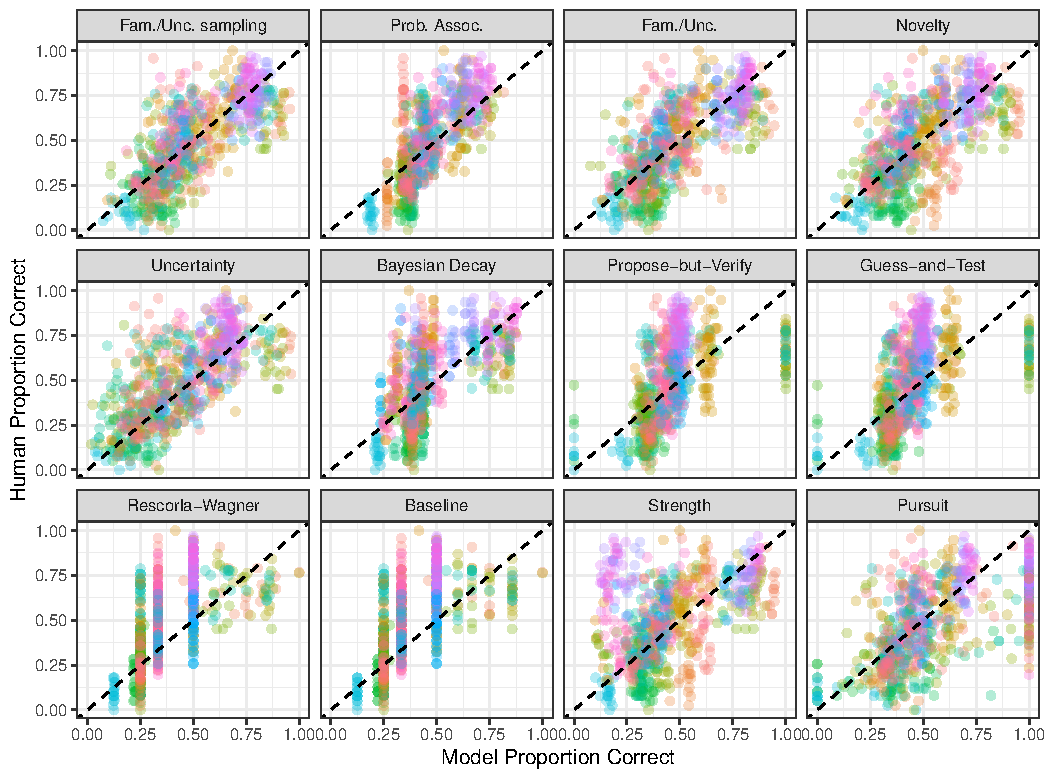
\includegraphics{figs/2-col-image-1} 

}

\caption[Human vs]{Human vs. model item-level accuracy using best-fitting parameters per model for all conditions (colored by condition). Note that on some items, PbV, GnT, and Pursuit all show more extreme responding (1 or 0) than people ever do.}\label{fig:2-col-image}
\end{figure*}
\end{CodeChunk}

\hypertarget{generalization-experiment-results}{%
\subsection{Generalization Experiment
Results}\label{generalization-experiment-results}}

Using the optimal parameters found for each model in the group fit, we
simulated model performance for four other published (two adult, two
developmental) for which we only have participants' average performance.
Koehne, Trueswell, \& Gleitman (2013) manipulated the temporal order
with which words were assigned two meanings of different strengths
across four conditions given to adults. Medina et al. (2011) manipulated
the informativeness (number of referents per trial) and order of trials
across four conditions, again with adults. The pattern of results from
both of these experiments were seen as evidence that people learn via
hypothesis testing, but we find that the Koehne et al.~data is best
accounted for by the novelty-biased model, and the Medina et al.~data is
best predicted by the Rescorla-Wagner model. L. B. Smith \& Yu (2008)
and Yu \& Smith (2011) trained 12- and 14-month-old infants on 6 words
repeated across 30 trials, and found that infants learned 4 words on
average. Suanda et al. (2014) tested 6-year-old children in three
conditions with varying contextual diversity. Table 3 shows the
root-mean-square error (RMSE) of each model vs.~average human
performance, as well as the total RMSE separately for the adult
experiments and the developmental experiments. The models generally
outperformed children and thus did not fit well to the developmental
conditions. Nevertheless, the Rescorla-Wagner model best matched both
the Medina et al.~adult data and the Smith \& Yu developmental data. The
novelty-biased model best predicted the Koehne et al.~adult data, with
FUs and the Strength-biased models just behind. Finally, the Suanda et
al.~developmental data was best fit by the Bayesian Decay model.

\begin{table}
\centering
\caption{\label{tab:gen-exp-table}Generalization experiment results.}
\centering
\resizebox{\ifdim\width>\linewidth\linewidth\else\width\fi}{!}{
\begin{tabular}[t]{lllllll}
\toprule
Model & Koehne & Medina & Suanda & Smith \& Yu & Adult RMSE & Dev RMSE\\
\midrule
baseline & 0.09 & \textbf{0.1} & 0.11 & \textbf{0.17} & \textbf{0.19} & \textbf{0.28}\\
R-W & 0.09 & 0.11 & 0.11 & 0.17 & 0.2 & 0.28\\
Nov & \textbf{0.06} & 0.17 & 0.2 & 0.29 & 0.23 & 0.49\\
FUs & 0.08 & 0.16 & 0.25 & 0.27 & 0.24 & 0.52\\
Str & 0.07 & 0.17 & 0.18 & 0.29 & 0.25 & 0.47\\
\addlinespace
PA & 0.11 & 0.15 & 0.13 & 0.24 & 0.26 & 0.37\\
FU & 0.09 & 0.19 & 0.26 & 0.29 & 0.27 & 0.55\\
Unc & 0.1 & 0.19 & 0.2 & 0.22 & 0.29 & 0.42\\
GnT & 0.24 & 0.15 & 0.2 & 0.27 & 0.4 & 0.48\\
Pur & 0.15 & 0.25 & 0.28 & 0.24 & 0.4 & 0.53\\
\addlinespace
PbV & 0.25 & 0.16 & 0.21 & 0.28 & 0.41 & 0.49\\
BD & 0.15 & 0.45 & \textbf{0.05} & 0.32 & 0.6 & 0.36\\
\bottomrule
\end{tabular}}
\end{table}

\hypertarget{discussion}{%
\section{Discussion}\label{discussion}}

We set out to conduct a systematic comparison of several models of
cross-situational word learning models across a wide variety of
experimental conditions. Using a large dataset, we found best-fitting
parameters for 11 models both by simultaneously fitting all of the data,
and using cross-validation. The results of both fitting regimes were
consistent and clear: shown in Table 1, the associative models generally
achieved better fits (lower SSE and higher correlations) than the
hypothesis-testing models (GnT; Medina et al. (2011) and PbV; Trueswell
et al. (2013)), which made correlated predictions (see Table 2:
\(r=.65\)). However, it was also striking how similar many models'
predictions were, even to models representing disparate learning
theories.

The Rescorla-Wagner model, a prediction error-based associative model,
performed similarly to the GnT model, with highly correlated predictions
(\(r=.87\)), while PbV had the poorest fit, and made responses most
similar to the R-W model (\(r=.67\)). Moreover, the predictions of the
R-W model were also highly correlated with the baseline co-occurrence
counting model (\(r = .99\)): such similar predictions yielded by
seemingly different theories is surprising and warrants further
investigation. However, some models' particular patterns of responses
suggest certain theoretical shortcomings. For example, the hybrid
Pursuit model (Stevens et al., 2017) fared poorly, in part because it
often outperformed humans (\(M_{Pur} =\) 0.56, \(M_{hum} = 0.48\)).
Indeed, as shown in Figure 1, Pur, PbV, and GnT all showed a pattern of
inhuman responses: for a subset of items, the models either always got
them correct or always got them incorrect, while people were more
stochastic. And yet Pur made responses that were most highly correlated
with the FUs model (\(r=.74\))--one of the best-fitting models. In
summary, although the hypothesis testing models evaluated here did not
fare well, it is worth nothing that models from different theories can
often mimic each other--at least in some experimental conditions--and so
it is necessary to both 1) test other instances of general theories
(including hypothesis testing models with, say, a decaying memory to
reduce ceiling performance), and 2) use models to generate predictions
during experiment design, in order to choose more informative
experiments.

Among the associative models, the PA model (Fazly et al., 2010) and the
FU model (Kachergis et al., 2012) both fared quite well, and the
sampling version of the FU model (FUs) performed slightly better, albeit
with three free parameters compared to two in the PA model. The
predictions of the top three models were more correlated with each other
than with the human data (see Table 1): PA vs.~FUs: .87, PA vs.~FU: .84,
FU vs.~FUs: .92. But the PA model also showed a .84 correlation with the
Rescorla-Wagner model, and both FU and FUs showed a .87 correlation with
the simpler novelty-biased associative model (Nov)--stronger than for
the uncertainty-bias mechanism used by the FU models. Examining the
experimental conditions that were easiest for the models to fit can
indicate what types of designs are less useful to conduct to test
theories of learning. For example, the condition best accounted for by
six of the models had varied frequency (pairs appeared 3, 6, or 9 times)
with low contextual diversity (i.e., the words of each frequency
co-occurred only with each other): it turns out that showing a
performance advantage for more frequent items is straightforward for
many theories. Future work should aim to further explore when these
models make overlapping predictions, but another approach is to find
conditions where models make disparate predictions. The FUs and PA
models make maximally divergent predictions in the conditions with fewer
words than objects per trial (esp.~1 word x 3 referents and 1 word x 4
referents conditions), which hints at a difference in mechanism for
these models. A fruitful next step would be to use optimal experiment
design to generate a definitive experiment to differentiate these
models. Models also struggled with conditions that tested how learners
relax their bias for mutually exclusive pairings in the face of evidence
that two words may both map to two referents: five models had the worst
fit for conditions from Kachergis et al. (2012).

Although we have aimed for broad coverage of models and experimental
conditions, this study is far from complete in both respects. First,
there are many other models that we have not yet implemented (e.g.,
McMurray, Horst, \& Samuelson, 2012). Moreover, this dataset represents
performance from a fairly homogeneous sample: English-speaking US
college students. Future work should aim to include not only more
models, but a more broadly diverse sample, both in terms of language
background and age. The small number of generalization experiments run
here suggest that parameters fitted to adult experimental conditions do
not generalize well to developmental experiments: future research should
gather a larger set of developmental data and re-fit these models with
cross-validation. We invite other researchers to contribute datasets and
model implementations for future, larger-scale comparisons: data, model
code, and fitting procedures will be open-sourced and available on
\href{https://osf.io/s2aty/?view_only=c91c852f00b847e0a71d5f4deaf7b7a5}{OSF},
as well as through an R package \texttt{XSLmodels} which we invite other
to contribute to.

In summary, we have shown not only how a large model comparison can help
rank models from most to least able to account for human data, but also
how such comparisons can identify models that mimic each other, as well
as identifying experimental designs that might aid in distinguishing
models. Future work should extend this comparison to cross-situational
word learning models and extant datasets beyond those tested here, and
design novel experiments designed to distinguish these models. Finally,
assuming that cross-situational learning is an important tool in the
language learner's toolbelt, it is important to consider how these
models can be extended to incorporate other information sources at the
learner's disposal, such as social cues, pragmatics, and syntactic
constraints on meaning (Hirsh-Pasek, Golinkoff, \& Hollich, 2000;
Markman, 1990; Yurovsky \& Frank, 2017). While many of these models have
mechanisms for preferentially selecting and storing particular
associations, most have yet to formally incorporate relevant cues from
social partners--linguistic and nonlinguistic (though see Yurovsky \&
Frank, 2017). More broadly, we believe that structured model comparison
is a critical step towards developing more complete models and,
eventually, quantitative identification of the fundamental mechanisms of
word learning.

\hypertarget{references}{%
\section{References}\label{references}}

\hypertarget{refs}{}
\begin{CSLReferences}{1}{0}
\leavevmode\vadjust pre{\hypertarget{ref-Akhtar1999}{}}%
Akhtar, N., \& Montague, L. (1999). Early lexical acquisition: The role
of cross--situational learning. \emph{First Language}, \emph{19},
34--358.

\leavevmode\vadjust pre{\hypertarget{ref-Carey1978}{}}%
Carey, S., \& Bartlett, E. (1978). Acquiring a single new word.
\emph{Papers and Report on Child Language Development}, \emph{15},
17--29.

\leavevmode\vadjust pre{\hypertarget{ref-Clark1987}{}}%
Clark, E. V. (1987). The principle of contrast: A constraint on language
acquisition. In B. MacWhinney (Ed.), \emph{Mechanisms of language
aquisition}. Hillsdale, NJ: Erlbaum.

\leavevmode\vadjust pre{\hypertarget{ref-Fazly2010}{}}%
Fazly, A., Alishahi, A., \& Stevenson, S. (2010). {A Probabilistic
Computational Model of Cross-Situational Word Learning}. \emph{Cognitive
Science}, \emph{34}(6), 1017--1063.

\leavevmode\vadjust pre{\hypertarget{ref-Frank2009}{}}%
Frank, M. C., Goodman, N. D., \& Tenenbaum, J. B. (2009). Using
speakers' referential intentions to model early cross-situational word
learning. \emph{Psych. Science}, \emph{20}(5), 578--585.

\leavevmode\vadjust pre{\hypertarget{ref-Gleitman1990}{}}%
Gleitman, L. (1990). The structural sources of word meaning.
\emph{Language Acquisition}, \emph{1}, 3--55.

\leavevmode\vadjust pre{\hypertarget{ref-HirshPasek2000}{}}%
Hirsh-Pasek, K., Golinkoff, R. M., \& Hollich, G. (2000). An emergentist
coalition model for word learning: Mapping words to objects is a product
of multiple cues. In R. M. Golinkoff, K. Hirsh-Pasek, L. Bloom, L. B.
Smith, A. L. Woodward, N. Akhtar, \& G. Hollich (Eds.), \emph{Becoming a
word learner: A debate on lexical acquisition}. New York, NY: Oxford
University Press.

\leavevmode\vadjust pre{\hypertarget{ref-Kachergis2013nat}{}}%
Kachergis, G., \& Yu, C. (2013). More naturalistic cross-situational
word learning. In M. Knauff, M. Pauen, N. Sebanz, \& I. Wachsmuth
(Eds.), \emph{{Proc. of the 35th Annual Conference of the Cognitive
Science Society}}. Austin, TX.

\leavevmode\vadjust pre{\hypertarget{ref-Kachergis2017}{}}%
Kachergis, G., \& Yu, C. (2017). Observing and modeling developing
knowledge and uncertainty during cross-situational word learning.
\emph{IEEE Trans. On Cognitive and Developmental Systems}.

\leavevmode\vadjust pre{\hypertarget{ref-Kachergis2012gi}{}}%
Kachergis, G., Yu, C., \& Shiffrin, R. M. (2012). An associative model
of adaptive inference for learning word--referent mappings.
\emph{Psychonomic Bulletin and Review}, \emph{19}(2), 317--324.

\leavevmode\vadjust pre{\hypertarget{ref-Kachergis2016}{}}%
Kachergis, G., Yu, C., \& Shiffrin, R. M. (2016). A bootstrapping model
of frequency and contextual diversity effects in word learning.
\emph{Cognitive Science}.
http://doi.org/\href{https://doi.org/10.1111/cogs.12353}{10.1111/cogs.12353}

\leavevmode\vadjust pre{\hypertarget{ref-Koehne2013}{}}%
Koehne, J., Trueswell, J. C., \& Gleitman, L. R. (2013). Multiple
proposal memory in observational word learning. In \emph{{Proc. of the
35th Annual Meeting of the Cognitive Science Society}}.

\leavevmode\vadjust pre{\hypertarget{ref-Luce1959}{}}%
Luce, R. D. (1959). \emph{Individual choice behavior}. John Wiley.

\leavevmode\vadjust pre{\hypertarget{ref-Markman1990}{}}%
Markman, E. M. (1990). Constraints children place on word meanings.
\emph{Cognitive Science}, \emph{14}, 57--77.

\leavevmode\vadjust pre{\hypertarget{ref-Markman1992}{}}%
Markman, E. M. (1992). Constraints on word learning: Speculations about
their nature, origins and domain specificity. In M. R. Gunnar \& M. P.
Maratsos (Eds.), \emph{Modularity and constraints in language and
cognition: The minnesota symposium on child psychology} (pp. 59--101).
Hillsdale, NJ: Erlbaum.

\leavevmode\vadjust pre{\hypertarget{ref-mcmurray2012word}{}}%
McMurray, B., Horst, J. S., \& Samuelson, L. K. (2012). Word learning
emerges from the interaction of online referent selection and slow
associative learning. \emph{Psychological Review}, \emph{119}(4),
831--877.

\leavevmode\vadjust pre{\hypertarget{ref-Medina2011}{}}%
Medina, T. N., Snedeker, J., Trueswell, J. C., \& Gleitman, L. R.
(2011). How words can and cannot be learned by observation. \emph{PNAS},
\emph{108}(22), 9014--9019.

\leavevmode\vadjust pre{\hypertarget{ref-DEoptim}{}}%
Mullen, K., Ardia, D., Gil, D., Windover, D., \& Cline, J. (2011).
{DEoptim}: An {R} package for global optimization by differential
evolution. \emph{{J. Of Statistical Software}}, \emph{40}(6), 1--26.

\leavevmode\vadjust pre{\hypertarget{ref-Quine1960}{}}%
Quine, W. V. O. (1960). \emph{Word and object}. Cambridge, MA: MIT
Press.

\leavevmode\vadjust pre{\hypertarget{ref-Rescorla1972}{}}%
Rescorla, R., \& Wagner, A. (1972). A theory of pavlovian conditioning:
Variations in the effectiveness of reinforcement and nonreinforcement.
In \emph{Conditioning II: Current research and theory}.

\leavevmode\vadjust pre{\hypertarget{ref-Siskind1996}{}}%
Siskind, J. M. (1996). {A computational study of cross-situational
techniques for learning word-to-meaning mappings}. \emph{Cognition},
\emph{61}, 39--91.

\leavevmode\vadjust pre{\hypertarget{ref-Smith2010th}{}}%
Smith, K., Smith, A. D. M., \& Blythe, R. A. (2011). {Cross-situational
learning: An experimental study of word-learning mechanisms}.
\emph{Cognitive Science}, \emph{35}(3), 480--498.

\leavevmode\vadjust pre{\hypertarget{ref-Smith2008vg}{}}%
Smith, L. B., \& Yu, C. (2008). {Infants rapidly learn word-referent
mappings via cross-situational statistics}. \emph{Cognition},
\emph{106}, 1558--1568.

\leavevmode\vadjust pre{\hypertarget{ref-Stevens2017pursuit}{}}%
Stevens, J. S., Gleitman, L. R., Trueswell, J. C., \& Yang, C. (2017).
The pursuit of word meanings. \emph{Cognitive Science}, \emph{41},
638--676.

\leavevmode\vadjust pre{\hypertarget{ref-Suanda2014}{}}%
Suanda, S. H., Mugwanya, N., \& Namy, L. L. (2014). Cross-situational
statistical word learning in young children. \emph{{Journal of Exp.
Child Psych.}}, \emph{126}, 395--411.

\leavevmode\vadjust pre{\hypertarget{ref-Suanda2012}{}}%
Suanda, S. H., \& Namy, L. L. (2012). {Detailed behavioral analysis as a
window into cross-situational word learning}. \emph{Cognitive Science},
\emph{36}(3), 545--559.

\leavevmode\vadjust pre{\hypertarget{ref-Trueswell2013}{}}%
Trueswell, J. C., Medina, T. N., Hafri, A., \& Gleitman, L. R. (2013).
Propose but verify: Fast mapping meets cross-situational word learning.
\emph{Cognitive Psychology}, \emph{66}(1), 126--156.

\leavevmode\vadjust pre{\hypertarget{ref-Vlach2013}{}}%
Vlach, H. A., \& Johnson, S. P. (2013). Memory constraints on infants'
cross-situational statistical learning. \emph{Cognition}, \emph{127},
375--382.

\leavevmode\vadjust pre{\hypertarget{ref-Vlach2012eq}{}}%
Vlach, H. A., \& Sandhofer, C. M. (2012). {Fast mapping across time:
Memory processes support children's retention of learned words}.
\emph{Frontiers in Developmental Psychology}, \emph{3}(46), 1--8.

\leavevmode\vadjust pre{\hypertarget{ref-Yu2008}{}}%
Yu, C. (2008). A statistical associative account of vocabulary growth in
early word learning. \emph{Language Learning and Development},
\emph{4}(1), 32--62.

\leavevmode\vadjust pre{\hypertarget{ref-Yu2007}{}}%
Yu, C., \& Smith, L. B. (2007). {Rapid word learning under uncertainty
via cross-situational statistics}. \emph{Psych. Science}, \emph{18},
414--420.

\leavevmode\vadjust pre{\hypertarget{ref-yu2011you}{}}%
Yu, C., \& Smith, L. B. (2011). What you learn is what you see: Using
eye movements to study infant cross-situational word learning.
\emph{Developmental Science}, \emph{14}(2), 165--180.

\leavevmode\vadjust pre{\hypertarget{ref-yurovsky2017beyond}{}}%
Yurovsky, D., \& Frank, M. C. (2017). Beyond naïve cue combination:
Salience and social cues in early word learning. \emph{Developmental
Science}, \emph{20}(2), e12349.

\end{CSLReferences}

\setlength{\parindent}{-0.1in} 
\setlength{\leftskip}{0.125in}

\noindent

\bibliographystyle{apacite}


\end{document}
